\documentclass[12pt]{article}

%package to include pdf
\usepackage{pdfpages}

% For code listing
\usepackage{listings}
\usepackage{color}

% Another code listing package
\usepackage{minted}

% For links and hyperreferences
\usepackage{hyperref}
\hypersetup{
    colorlinks=true,
    linkcolor=blue,
    filecolor=magenta,      
    urlcolor=cyan,
}

\usepackage{subcaption}

% Wrapping text around figures (doesn't work)
\usepackage{wrapfig}
% Figures with side caption
\usepackage[rightcaption]{sidecap}
% Fancy header and footer package
\usepackage{fancyhdr}
\pagestyle{fancy}
\fancyhf{}
\fancyhead[R]{UON parser}
\fancyhead[L]{\rightmark}
%\fancyfoot[L]{\leftmark}
\fancyfoot[R]{\thepage}

\renewcommand{\headrulewidth}{0.5pt}
\renewcommand{\footrulewidth}{0.5pt}

\definecolor{mygreen}{rgb}{0,0.6,0}
\definecolor{mygray}{rgb}{0.5,0.5,0.5}
\definecolor{mymauve}{rgb}{0.58,0,0.82}

\lstset{ %
  backgroundcolor=\color{white},   % choose the background color
  basicstyle=\footnotesize,        % size of fonts used for the code
  breaklines=true,                 % automatic line breaking only at whitespace
  captionpos=b,                    % sets the caption-position to bottom
  commentstyle=\color{mygreen},    % comment style
  escapeinside={\%*}{*)},          % if you want to add LaTeX within your code
  keywordstyle=\color{blue},       % keyword style
  stringstyle=\color{mymauve},     % string literal style
}

% Set up data, if you need to add a package, go here
\input{setup/packages.tex}

\begin{document}


\thispagestyle{empty}
\setlength\headheight{0pt} 
\begin{center}

\begin{center}
\includegraphics[width=0.70\linewidth]{images/HEIG-VD_Logo.eps}            
\end{center}	

        %\vspace{0.25cm}
        %{\scshape\LARGE TU Dublin, Tallaght Campus \par}
        %\vspace{0.25cm}
        %{\scshape\Large BSc / HDip / MSc Project Template\par}
        %\vspace{0.5cm}
        \vspace*{\fill}
        {\Large\bfseries Parser for a serialization format UON™\par}
        
        \vspace{0.5cm}
        {\Large\itshape Stephane Selim\par}
        Department of TIC \\
        Orientation IL
        \vspace{0.25cm}

\vspace{1cm}
Subject proposed by\par
Prof. Yves Chevallier \\
Department of TIN\par

\vspace{1cm}
Supervised by\par
Prof. Yves Chevallier \\
Department of TIN\par

\vspace{1cm}
Academic Year\par
2019-2020\par

\large
\vfill
\begin{flushright}
Yverdon-les-Bains, \today
\end{flushright}

\vspace*{\fill}
\end{center}

\clearpage
\restoregeometry
\justify

\vspace*{\fill}
\begin{center}
\section{Foreword}  
This Bachelor project (hereinafter TB for "Travail de Bachelor") is carried out at the end of the school curriculum, in preparation for obtaining the title of Bachelor of Science HES-SO in Engineering.

As an academic work, its content, without prejudging its value, engages neither the responsibility of the author, nor that of the jury of the Bachelor project and the School.

Any use, even partial, of this TB must be made in accordance with copyright.

\vfill
\begin{flushright}
HEIG-VD

Dean name: Vincent Peiris \break
Head of TIC Department
\end{flushright}

\vfill
\begin{flushleft}
Yverdon-les-Bains, \today
\end{flushleft}

\end{center}
\vspace*{\fill}

\pagebreak

\vspace*{\fill}
\begin{center}
\section{Declaration}

I, the undersigned Stephane Selim, hereby certifies having carried out this work alone and having not used any other source than those expressly mentioned.

\vfill
\begin{flushleft}
Yverdon-les-Bains, \today
\end{flushleft}

\vfill
\begin{flushright}
Stephane Selim
\end{flushright}

\end{center}
\vspace*{\fill}

\pagebreak

\tableofcontents
\pagebreak

\section{Introduction}
The following Bachelor project consists of implementing a parser for the newly created serialization language UON (which stands for Unified Object Notation). In the following, we will present the motivation behind this new serialization language, the specification for this language and how we went about implementing a parser for it. In detail, we will see the incentive behind designing a new serialization language in an already crowded field, we will see what makes it stand out among the others well known like JSON, XML or YAML and how it accomplishes specific needs compared to the others. We will present the key aspects of the specification of the language. We will then present the implementation, the tools and the choices we’ve taken at every stage of the parser, starting with the grammar of the language to the processing of the final resulting AST (Abstract Syntax Tree).

\pagebreak

\section{Pre-Study}
UON is a newcomer to the field of data serialization. To understand how UON stands out among its already established peers like JSON or YAML, we need to delve into the world of serialization and have a look at what serialization does and what UON offers that others don’t.

\subsection{Serialization}
We live in a heterogeneous world where data is constantly moved and transferred from one endpoint to another. But the way these endpoints interpret the data and store it is not the same from one another. So we need some way to send the data that is platform and language-agnostic. We need to \textbf{serialize} the data, that is transform it into a format that can be understood by all platforms. This is the main reason we serialize data for.

For example, say we have a Java class Person with attributes name and age. A Java object of this class would be as follows:

\begin{lstlisting}[language=java]
Person person = new Person("Fred", 28);
\end{lstlisting}

Now you need to send that data over to another endpoint that only runs on Python. How would you go about sending that data onto the network and how do you expect Python to interpret it? Python only understands Python classes and you’re sending him a Java Object.
Here is when serialization comes in handy. You make the Java class Person \emph{Serializable} (by implementing its interface) and you translate the object into some serialization format such as the well-known JSON:

\begin{lstlisting}{language=json}
{
  Person: {
    "name": "Fred",
    "age": 28 
  }
}
\end{lstlisting}

\hfill\break
Or XML: 

\begin{lstlisting}[language=xml]
<Person>
  <name> Fred </name>
  <age> 28 </age>
</Person>
\end{lstlisting}

and you send it over the network. When Python receives the data, he \emph{deserialize}s it to rebuild the original data, now as a Python object of type Person of which you already created a Python class for it.

\subsubsection{Definition}
More formally, from the definition taken from the microsoft Docs, \textbf{serialization} can be defined as the process of storing the state of an object to a storage medium. During this process, the public and private fields of the object and the name of the class, including the assembly containing the class, are converted to a stream of bytes, which is then written to a data stream. When the object is subsequently deserialized, an exact clone of the original object is created. It can be used as we said when we want to transfer data over a network, or when we want to store data on a medium such as hard disks or databases or any other situation where you’d want to store data in a format that is independent of the architecture or the platform.

\begin{figure}[ht!]
 	\centering
 	\caption{Serialization process}
 	\includegraphics[width=0.7\linewidth]{images/Serialization/serialization_illustration.eps}
 	\label{lab:perceptron}
\end{figure}

So when we said that Java objects can be serialized as in the previous example, we weren’t entirely accurate. In the previous example, we converted the object to a JSON object, which of course you can, but Java also has its own internal serialization process. The java object to be serialized must implement the interface \emph{java.io.Serializable} (or its subinterface \emph{java.io.Externalizable} if you want more control of how serialization is done on your object), this flags the class as valid for serialization. Then you can use an \emph{OutputStream} to write the data of the object of this class to a file or to a socket. The output will be a byte stream so you can’t really read it with your eyes but it will contain all the data of the object, as well information on the class itself. So it can now be effectively read by another computer or another program and correctly reconstruct the data.

Here is another example that I find very illustrative:

\begin{figure}[ht!]
 	\centering
 	\caption{Serialization process}
 	\includegraphics[width=3cm, height=8cm]{images/Serialization/serialization_image_example.png}
 	\label{lab:perceptron}
\end{figure}

When you send an image over the internet, the same process happens. The image and its data are serialized. Just as the way you store an image in SQL database, you save it in a Blob, which is essentially converting the image into a stream of bytes (hence the name Binary large object).


% \begin{wrapfigure}{r}{0.5\textwidth}
%   \begin{center}
%     \includegraphics[width=0.48\textwidth]{images/Serialization/serialization.png}
%   \end{center}
%   \caption{Birds}
% \end{wrapfigure}

\subsection{Serialization formats}
When you serialize the data, we’ve seen that you can serialize in either binary format or in a text format. So the question you would want to ask yourself is why choose one over the other and what advantages does this have?

Text format is human-readable, which is in itself a big plus. In contrast, binary format is generally faster to process, which is endemic to binary encoding itself. Binary content is more compact than its text counterpart since the latter required more bytes. Thus we find ourselves with increased performance and efficiency of access when working with binary.

\subsection{Benchmarks}\label{benchmarks}
To test the difference in performance between binary and text format serialization, we’ve run a small benchmark test done in Python, between binary formats like BSON and Msgpack, and text formats like JSON and YAML, on the following data :

\begin{lstlisting}[language=python]
data = {
   "name": "Jack",
   "age" : 28,
   "hobbies" : ["skating", "eating", "jogging"],
   "description": """Lorem ipsum dolor sit amet, consectetur adipiscing elit, sed do eiusmod tempor incididunt ut
               labore et dolore magna aliqua. Ut enim ad minim veniam, quis nostrud exercitation ullamco laboris nisi
               ut aliquip ex ea commodo consequat. Duis aute irure dolor in reprehenderit in voluptate velit esse cillum
               dolore eu fugiat nulla pariatur. Excepteur sint occaecat cupidatat non proident, sunt in culpa qui officia
               deserunt mollit anim id est laborum. """
}
\end{lstlisting}

 We’ve used the official Python libraries for each of these formats to run these tests. Here are the results (measured in seconds as a float) of 10000 iterations for each test:
 \hfill\break

\subsubsection{BSON}
\begin{lstlisting}[language=python]
 s = '''
 a = bson.dumps(data)
 b = bson.loads(a)
 '''
 print("BSON time: ", timeit.timeit(setup=mysetup, stmt= s, number=10000))
\end{lstlisting}

Using \href{https://github.com/py-bson/bson}{bson from py-bson}
We get BSON time:  0.91669s.

\subsubsection{JSON}
\begin{lstlisting}[language=python]
  s_json = '''
 a = json.dumps(data)
 b = json.loads(a)
 '''
 print("JSON time: ", timeit.timeit(setup=mysetup_json, stmt= s_json, number=10000))
\end{lstlisting}

Using the in-built module \href{https://docs.python.org/3/library/json.html}{json}
We get JSON time:  0.20858s.

\subsubsection{Msgpack}
\begin{lstlisting}[language=python]
 s_msgpack = '''
 a = msgpack.packb(data, use_bin_type=True)
 b = msgpack.unpackb(a, raw=False)
 '''
 print("MsgPack time: ", timeit.timeit(setup=mysetup_msgpack, stmt= s_msgpack, number=10000))

\end{lstlisting}

Using the \href{https://github.com/msgpack/msgpack-python}{msgpack module}
We get MsgPack time:  0.070190s.

\subsubsection{YAML}
\begin{lstlisting}[language=python]
 s_yaml = '''
 a = yaml.dump(data)
 b = yaml.load(a, Loader=yaml.FullLoader)
 '''
 print("YAML time: ", timeit.timeit(setup=mysetup_yaml, stmt= s_yaml, number=10000))

\end{lstlisting}

Using the \href{https://pyyaml.org/wiki/PyYAMLDocumentation}{PyYAML module}
We get a whopping YAML time:  41.1645s!

We see that MsgPack has the fastest time compared to the second best JSON, with a factor of 2 or 3 times as fast, which is due to the binary serialization of msgPack. By contrast YAML, which is the most human readable of them all,  has the slowest recorded performance with a factor of at least 200x slower than JSON’s! This is due to the inherent complexity of the YAML specification which translates into its parsers as well.

One small inconsistency that we noticed is BSON’s performance. BSON is binary serialization and while it’s still fast, it records performance time slower than that of JSON’s. Why? Well this is probably not due to the format itself but to the environment in which it is executed. We’ve run these tests in Python but this problem was also present in Node.js \href{https://stackoverflow.com/questions/36767310/why-is-json-faster-than-bson-in-node-js}{[2]}. In most environments, binary encodings would be easier to encode but some formats like JSON have in-built serialization in the environment that is implemented in native code and in an optimised fashion. This might be what is happening in Python as well. The in-built \emph{json} module might be more optimised than bson’s python module (which is actually an Independent BSON codec for Python that doesn’t depend on MongoDB’s BSON). This explains the difference in performance between the two formats in this particular case.

As a rule of thumb, if you’re looking for a format that is heavy on performance and requires less storage space, binary serialization might be what you’re looking for. Otherwise you’re better off with text based format, especially when you’re constantly checking your data, for example during debugging, and you don’t want to go through other tools to be able to read your data.

\pagebreak

\subsection{Overview of some serialization formats}

\subsubsection{JSON}
JSON (JavaScript Object Notation) is a lightweight data-interchange text-format that is based on a subset of the JavaScript Programming Language. Since JavaScript is used across the web, this makes JSON the de facto leader of serialization formats when it comes to web applications. \href{https://www.json.org/json-en.html}{[3]}

It has dominated the field with its minimal and human-readable format. It has become an alternative to the well-established XML as a way of transmitting data between servers and web applications. Developers love it for its simplicity and its structuring of data.

It is built on two structures:
\begin{itemize}
    \item A collection of key/value pairs. This represents an equivalent data structure in most programming languages like Maps in Java or dictionaries in Python.
    \item An ordered list of values. This also represents an equivalent data structure in most programming languages like lists, sequences or arrays (which represent the same thing: an ordered set of values, with each having its own index in the structure).
\end{itemize}

The representation of these structures mimic those of Python. Given these two simple structures, the format has a very simple syntax grammar and most programming languages are equipped with parsers for this format. The simplicity of this format has allowed some of the parsers to be very well optimized, like JavaScript which is natively optimized for dealing with JSON. 

Example:
\begin{minted}{json}
{
  "firstName": "John",
  "lastName": "Smith",
  "age": 27,
  "address": {
    "streetAddress": "21 2nd Street",
    "city": "New York",
  } ,
 "children": [],
  "hobbies": ["Jogging", "Reading"]
}
\end{minted}

Notes: Data structures can be nested. Strings need to be delimited with double-quotes and support backslash escaping syntax. It doesn’t support comments however.

\subsubsection{YAML}
Yaml, short for Yet Another Markup Language originally, and then retconned later to be a recursive acronym for YAML Ain't Markup Language,  referring more accurately to its purpose of data serialization rather than a mere document markup format. 
YAML has taken the step forward to be more human-readable than JSON. It’s so human-readable that they made the home page of YAML in YAML \href{https://yaml.org/}{[4]}. But this comes at a cost of a much, much bigger specification and grammar complexity. They have already gone through three specifications. They are currently at YAML 1.2, which added compliance with JSON as an official subset. That means that as of YAML 1.2, JSON will be recognized as valid YAML.

It features 3 primitives: mapping (hashes/dictionaries), sequences (arrays, lists) and scalars (strings/numbers). YAML leverages these primitives, and adds a simple typing system and aliasing mechanism to form a complete language for serialization of any native data structure. While most programming languages can use YAML for data serialization, YAML excels in working with those languages that are fundamentally built around the three basic primitives. It also uses whitespace indentation (like Python) to indicate nesting so there is no need for quotes or brackets which makes it more compact.

Owing to its readability and its compact form, it has become widely used, for example for writing configuration files, with tools such as Ansible or Docker adopting the format to write their configuration files.

It also comes with a wide range of parsers in many languages, each one more complicated as the other, to keep up with the format complexity and its defined types. Creating a fully compliant parser with YAML has proven almost impossible \href{https://github.com/yaml/yaml-grammar}{[5]}. This will almost certainly be reflected in the implementation of a parser for UON, the format of which very closely resembles YAML.

Here is an example:

\begin{lstlisting}
- name: John Smith
  age : 27
  address:
     streetAddress :  21 2nd Street
     city: New York
  hobbies: [Jogging, Reading]
- {name : Maggie Smith,
   age : 28}
\end{lstlisting}

\subsubsection{XML}
XML (eXtensible Markup Language) appeared in the mid-1990s as a successor to SGML ( Standard Generalized Markup Language).  Best known for its use in the web early on. It is strictly text-format, but a binary XML version has been proposed to have a more compact format.\href{https://www.w3.org/2003/08/binary-interchange-workshop/29-MicrosoftPosition.htm}{[6]}

XML is a markup format based on tags. Each XML document contains one or more elements, the boundaries of which are either defined by <start-tags>, <end-tags> or empty-element tag for empty elements. Each starting tag must be closed by a closing tag and tags can contain attributes. Elements can contain other elements. This gives a logical structure to the document.
XML can also be validated using a schema like DTD (document type definition) that defines grammatical rules that the XML document must follow. 

Here is an example:
\begin{minted}{xml}
<People>
   <Person>
      <name>John Smith</name>
      <age>2</age>
      <address category="nested">
         <street>21 2nd Street</street>
         <city>New York</city>
      </address>
   </Person>
   <Person>
      <name>Maggie Smith</name>
      <age>28</age>
   </Person>
</People>
\end{minted}

The format is well-formed but, as you may have noticed, it is very verbose and redundant, which is a well-known downside of XML with restrictions such as opening tags must be closed. It is still a text human-readable format but less so compared to others. You can easily get lost between the tags when reading an XML document. The added level of sophistication of this format can also be seen in its parsers, when trying to translate it into code objects. Speaking from personal experience, it can get quite tricky especially with XML elements that come with attributes.

We see it slowly being replaced by the much more concise and simple JSON, since developers will almost always value simplicity over anything else. 

\subsubsection{BSON}
BSON (“Binary JSON”) is a binary serialization format \href{http://bsonspec.org/spec.html}{[7]}. It has been developed internally by MongoDB \href{https://www.mongodb.com/json-and-bson}{[8]} and Mongo uses it as a data storage and network transfer format for its database. But it can also be used outside MongoDB.

It is basically the binary encoding of JSON-like documents (which are UTF-8 String encoded). So it still keeps the ordered key/values pairs structure, but everything is binary. Apart from encoding, it also keeps the length information of the document to make the document traversal when parsing it faster. It supports numeric types that are not native to JSON, representing different precisions such as int32, int64, uint64, double or decimal128. This is convenient when parsing in a language that supports these different sized integers.  It also adds more native types like the “BinData” data type to represent an array of bytes.  

Here are examples taken from the MongoDB’s “JSON and BSON” page when serializing some basic data structures from languages like JavaScript and Python :

\begin{figure}[ht!]
 	\centering
 	\caption{Binary Serialization with BSON 1}
 	\includegraphics[width=0.7\linewidth]{images/Serialization/BSON_example_1.png}
 	\label{lab:perceptron}
\end{figure}

\begin{figure}[ht!]
 	\centering
 	\caption{Binary Serialization with BSON 2}
 	\includegraphics[width=0.7\linewidth]{images/Serialization/BSON_example_2.png}
 	\label{lab:perceptron}
\end{figure}

\subsubsection{Protocol Buffers}
Another example of the well-known binary serialization formats are Google’s Protocol buffers, Protocol buffers are a language-neutral, platform-neutral, extensible mechanism for serializing structured data \href{https://developers.google.com/protocol-buffers}{[9]}. There’s not a better way to explain what PBs are except to cite Google’s Protocol Buffers page itself: “Protocol buffers are a flexible, efficient, automated mechanism for serializing structured data – think XML, but smaller, faster, and simpler. You define how you want your data to be structured once, then you can use special generated source code to easily write and read your structured data to and from a variety of data streams and using a variety of languages. You can even update your data structure without breaking deployed programs that are compiled against the "old" format.”

First you specify how you want your serialized data to be structured in \emph{.proto} files which have a specific format you have to respect. Here is an example of one such file: 

\begin{lstlisting}
message Person {
  required string name = 1;
  optional string nickname = 2;
  required int32 age = 3;

  message Address {
    required string street = 1;
    optional string number = 2;
  }
}
\end{lstlisting}

message Person {
  required string name = 1;
  optional string nickname = 2;
  required int32 age = 3;

  message Address {
    required string street = 1;
    optional string number = 2;
  }
}

Each protocol buffer message is a small logical record of information containing a series of uniquely numbered fields, one for each piece of data you want to include in that type of message. Each field has a name and a value type. The unique number of the fields is used to identify them in the message binary format. You can specify \emph{required} fields, \emph{optional} fields and \emph{repeated} fields. You can nest messages inside others to have a hierarchical structure. The scalar fields like the ones in the example above are of type string or int32. But Protocol Buffers also supports a multitude of data types with different precisions such as int64, uint32, uint64, double, float and so on \href{https://developers.google.com/protocol-buffers/docs/proto#scalar}{[10]}. When a message is encoded, the keys and values are concatenated into a byte stream. On the receiving-end of a protocol buffer message, the decoding apparatus references the \emph{.proto} file to reconstruct the original message. 

Since it’s binary, protocol buffer serialization is fast. As Google draws the comparison with XML, it is 3 to 10 times smaller, 20 to 100 times faster and less ambiguous than XML. It can also generate data access classes that are easier to use programmatically which is very convenient for the developer that wants to work with this data when he receives it. For instance with the example above, compiling the \emph{.proto} file would generate a Person class with attributes for name, nickname and age and would define getters and setters for it.

\subsection{Performance comparison}

The following is the result of some of the benchmark tests done by other people that I found on the internet, to compare the speed and size performance of a selection of serialization formats. These were not performed by me on my local computer so there is no way to verify them and should always be taken with a grain of salt. However the results correspond more or less to the actual performances of these serialization formats and the conclusions drawn by me. Please refer to subsection \ref{benchmarks} for the benchmark tests that were run by me on my local computer, on Python.

The following tests were done in \href{https://blog.mbedded.ninja/programming/serialization-formats/a-comparison-of-serialization-formats/#speed-comparison-benchmarking}{this 2019 blog}, so they are still fairly new at the time of writing this report. It compares the speed and file size between JSON, XML, protocol buffers, TOML, YAML and CSV (which is still considered a serialization format used to represent data). The serialization/deserialization is done using libraries for each of these formats in Python and C++. The sample data to be serialized consists of a \emph{vector} in C++ or a \emph{list} in Python of a \emph{Person} data structure (or class in Python).

\begin{figure}[h]

\begin{subfigure}{0.4\textwidth}
\includegraphics[width=0.9\linewidth, height=5cm]{images/Performance Comparison/mbedded_ninja_performance_c.png} 
\caption{C++ performance comparison}
\label{fig:subim1}
\end{subfigure}
\hfill
\begin{subfigure}{0.4\textwidth}
\includegraphics[width=0.9\linewidth, height=5cm]{images/Performance Comparison/mbeded_ninja_performance_python.png}
\caption{Python performance comparison}
\label{fig:subim2}
\end{subfigure}
\caption{Serialization and deserialization comparison}
\label{fig:image2}
\end{figure}

As we’ve seen the speed comparison results correspond more or less to those that we’ve got above in subsection \ref{benchmarks}. YAML, as to its complexity, takes a huge amount of time compared to others.  And after comes TOML which is also a YAML-like serialization format that aims to be very human-readable at the cost of complexity of its structure. Protocol buffers as expected have very good performance in both programming languages. Now the results of these tests have been taken from the minimum of several runs, and the results can also vary depending on the library used for a serialization format. A performance degradation from one programming language to another may be inherent to the language (C code being a lot faster than Python) or just a case of a badly written serialization library. 
But this gives a general idea of the performance of different serialization formats, and how the complexity of a serialization format is reflected into its performance.

This was only an overview of some of the serialization formats that are available today. We went over the most used and which ones people are most likely to use in their serialization needs and applications, but there are a lot more out there that suit different needs. For a more comprehensive view over the ensemble of the formats, Wikipedia provides a very good and exhaustive comparison between a lot of serialization formats, on certain points and features like binary support or human-readability. \href{https://en.wikipedia.org/wiki/Comparison_of_data-serialization_formats}{[11]}

\pagebreak

\subsection{UON}
We’ve seen the most used serialization formats, what really defines them and makes them stand out amongst others, as well as some of their shortcomings. UON (short for Unified Object Notation) is a new proposed serialization format that seeks to regroup the best features of these serialization formats into one format that encompasses them all. 

\subsubsection{Why UON?}
The main motivation behind UON is to serve the needs of \href{https://en.wikipedia.org/wiki/Industry_4.0}{Industry 4.0}, the 4th revolution that has occurred in the industry. It is not just a buzzword, it is actually happening all around us where traditional practises of the industry are replaced by the latest smart technology within the large scale m2m (machine to machine) communication and Internet of Things (IoT) deployments. This increased automation is shown in the huge amount of computers that are connected and communicate with one another to make decisions without human intervention. This process incurs a huge amount of information and data that are circulated around and the machines involved usually have very limited computation power (we’re not talking about full-blown pc with an ssd and ram, we’re talking about small devices like sensors and controllers and such). 

This begs for some serialization format that could be convenient for encapsulating and representing that data, in the smallest payload possible.
UON hopes to fill this need. Other serialization formats may fulfill specific needs:  JSON with its simplicity satisfies the Web APIs developers, protocol buffers with its concise binary format, interoperability and schema validation, but UON aims to be ubiquitous covering a wide range of applications from battery-powered telemetry sensors to Web communication protocols. For that UON defines a way to :

\begin{itemize}
  \item encode/decode payloads written in binary or in human-readable form
  \item Describe a payload through a validation schema
\end{itemize}

\subsubsection{What is UON?}
UON is a data serialization format. It is meant to be UTF-8 encoded by default, but compatible with other encoding standards. It is built upon concepts described by C, Perl, Python, Ruby, JSON and YAML. Let’s go over some of the most important features of UON.

\textbf{Note: Starting from now and until the end of this document, all written \emph{UON} and/or \emph{UON} excerpts will be formatted (unless it's just plain \emph{JSON} in which case we will be using \emph{JSON} formatting). Since there is no official \emph{UON} formatting yet, we will be using Python formatting.}

\subsubsection{Design}
UON is designed to be a superset of JSON. It features four levels of complexity and each of them adds more features.

\begin{itemize}
    \item \textbf{UON:0} is strictly speaking JSON, keywords have to be double quoted, comments are not permitted and well, it is simply JSON.
    \item \textbf{UON:1} encompasses some of the YAML standards. It is a reduced set of YAML.
    \item \textbf{UON:2} adds type properties which allow you to qualify a type, for instance by setting the base of a number !int(base:36) ah1ddb1.
    \item \textbf{UON:3} extends UON:2 by adding extended types and syntaxic sugars to simplify the readability.
\end{itemize}

\begin{figure}[ht!]
 	\centering
 	\caption{UON complexity levels}
 	\includegraphics[width=0.7\linewidth]{images/UON/complexity-levels.png}
 	\label{fig:Complexity levels}
\end{figure}

So while UON is fully compliant with JSON, it is partially compliant with YAML. The full compliance with JSON is so that those who are familiar with JSON may feel at home, while still making the best out of the rest of the UON features. The partial compliance with YAML stems from YAML features that may make UON unnecessarily complicated.

Here is another figure that better illustrates the compliance of UON with JSON and YAML:

\begin{figure}[ht!]
 	\centering
 	\caption{UON supersets}
 	\includegraphics[width=0.7\linewidth]{images/UON/supersets.png}
 	\label{fig:UON supersets}
\end{figure}

Here is an example of UON:3
\begin{lstlisting}[language=python]
{
  person(desc: "A person"): {
    name: !str(length: 42, pattern: /[A-Za-z ]+/) "John Doe"
    age: !int(base:4, dictionary: ["Ga", "Bu", "Zo", "Meu"]) "Ga Ga Zo Meu Bu"
  }
}
\end{lstlisting}

And here is the equivalent JSON format:

\begin{minted}{json}
{
  "key": "person",
  "properties": {
    "desc": "A person"
  },
  "value": {
    "name": {
      "type": "str",
      "properties": {
        "length": 42,
        "pattern": {
          "type": "regex",
          "value": "[A-Za-z ]+"
        },
      },
      "value": "John Doe"
    },
    "age": {
      "type": "int",
      "properties": {
        "base": 4,
        "dictionary": ["Ga", "Bu", "Zo", "Meu"],
      },
      "value": "Ga Ga Zo Meu Bu"
    }
  }
}
\end{minted}

\subsubsection{Information model}
To have a good idea of the resemblance between YAML and UON, let’s take a look first at YAML’s information model.
\url{https://yaml.org/spec/1.2/spec.html}. 

The YAML information is used in two ways: for machine processing, and for human consumption. Parsing YAML (\emph{Load}) or serializing data to YAML (\emph{Dump}) is a quite complicated process and it involves a tool called a \emph{processor}. The processor is responsible for reconciling between these two complementary views.The processing of YAML information is done in three stages: \textbf{Representation}, \textbf{Serialization} and \textbf{Presentation} as shown in the figure below:

\begin{figure}[ht!]
 	\centering
 	\caption{YAML Process stages}
 	\includegraphics[width=0.7\linewidth]{images/UON/YAML_process_stages.png}
 	\label{fig:YAML processor}
\end{figure}

\href{https://yaml.org/spec/1.2/spec.html#representation//}{Representation} addresses how YAML views \href{https://yaml.org/spec/1.2/spec.html#native data structure//}{native data structures} to achieve portability between programming environments. This is the first stage when serializing native data structures to YAML (going from left to right in the figure above). YAML represents any native data structures using three kinds of structures or \emph{nodes}, namely:

\begin{itemize}
    \item \emph{Collection nodes}: \textbf{sequence}, \textbf{mapping}
    \item \textbf{scalar}  (any datum with opaque structure presentable as a series of Unicode characters or simply put a \emph{string}).
\end{itemize}

After this stage, we end up with a node Graph, where each node contains information necessary to reconstruct the original native data structures.

\href{https://yaml.org/spec/1.2/spec.html#serialization//}{Serialization} concerns itself with turning a YAML representation into a serial form, that is, a form with sequential access constraints. This involves imposing an ordering on mapping keys and to replace the second and subsequent references to a given node with place holders called aliases. This eases human friendly key order. The result of this stage is a serialization tree, that can then be traversed to produce a series of event calls for one-pass processing of YAML data. More on that later.

\href{https://yaml.org/spec/1.2/spec.html#presentation//}{Presentation} deals with the formatting of a YAML serialization as a series of characters in a human-friendly manner, such as node styles (double quote scalars, explicit json-style mappings, etc…), the amount of indentation and others. While some of this can be done with the help of the application, in general this process should be guided by the preferences of the user.

A YAML processor need not expose the serialization or representation stages. It may translate directly between native data structures and a character stream (\emph{dump} and \emph{load} in the diagram above). However, such a direct translation should take place so that the native data structures are constructed only from information available in the representation.

The following diagram summarizes the three information models. Full arrows denote composition, hollow arrows denote inheritance, “1” and “*” denote “one” and “many” relationships. A single “+” denotes serialization details, a double “++” denotes presentation details. 
\begin{figure}[ht!]
 	\centering
 	\caption{YAML information model}
 	\includegraphics[width=0.7\linewidth]{images/UON/YAML_information_model.png}
 	\label{lab:perceptron}
\end{figure}

\textbf{UON information model}

\begin{figure}[ht!]
 	\centering
 	\caption{UON information model}
 	\includegraphics[width=0.7\linewidth]{images/UON/information_model_updated.png}
 	\label{lab:perceptron}
\end{figure}

Each item in UON that composes UON object tree is a \emph{Type} that may have several properties. 
We see the familiar collection and scalar nodes from the representation stage of YAML.
Three kind of properties exist:
\begin{itemize}
    \item Presentation properties: Presentation properties are any properties that influence the presentation of a value, such as !seq(orderd: true) [9, 8, 7] a resolved payload will be [7, 8, 9].
    \item Validation properties: Validation properties are used to validate, constrain and describe a UON file.
    \item Application properties: These properties can only be read from UON using the \emph{!prop} type. They are accessible from the application (Python, JavaScript, ...). They are used to generate a serialized file (binary, or UON), but they are never explicitly passed.
\end{itemize}

\subsubsection{Validation}
One of UON’s strongest features is validation according to some schema. In the context of Industry 4.0, validating transmitted data between machines with very limited computation power is a big plus. 

When two devices want to exchange information they have two communication channels:
\begin{itemize}
    \item An online communication channel used for payload data transmission
    \item A contractual communication channel used for schema agreement
\end{itemize}

Take for instance the following example:

In the following figure, we have on the left, two devices: a low power temperature sensor, and a powerful home automation gateway. To reduce the payload size, both devices agree on a schema which describes the payload format.

\begin{figure}[ht!]
 	\centering
 	\caption{Home automation data exchange and schema refining}
 	\includegraphics[width=0.7\linewidth]{images/UON/home_automation_data_exchange.png}
 	\label{lab:perceptron}
\end{figure}

On the right side of the figure, the generic schema that describes a temperature sensor is \textbf{refined} by narrowing the schema for instance by saying the generic temperature expressed with a number, is now an unsigned eight bit value expressed in Celsius degrees.

Some serialization formats offer validation such as XML with XSD (XML Schema Definition), or JSON Schema which is separate from JSON, but allows to annotate and validate JSON documents or even \emph{.proto} files in protocol buffers (\emph{.proto} files are required for the latter, and though they allow validation, that is not their main purpose).

A UON’s validation schema is still UON. Here is an example of a validation schema for a Person data structure:

\begin{lstlisting}
# Person schema
!!person: {
  firstname: !str(pattern=/[A-Z][a-z]+/),
  lastname: !str(min: 2, max: 32),
  age: !uint(min: 7, max: 77, desc: "Age of the person that is able to play table games")
}
\end{lstlisting}

The schema defines a set of constraints that the attributes of a Person must follow in order to be validated. In this case we set the types of \emph{firstname} and \emph{lastname} as strings, with \emph{firstname} defined by a regular expression that constrains it to start with a Capital letter, \emph{age} as an unsigned integer, with values in the range of [7, 77].

\subsubsection{Shortcomings}
TODO
UON provides a lot of native types. But it also provides a way for users to define their own types using schemas. Usually
UON aims to be very complete. If there's a feature you would like a serialization language to have, UON probably has it. This means that if you're going to build a parser for it, it will not be an easy feat, as witnessed by the uon-parser Python implementation accompanying this project. As mentioned before, with a complicated specification such as YAML's, it logically follows that its parser will be as, or even more, complicated for it to really follow and comply with the specification. Usually in the case of YAML parsers, the parser will introduce some compromise while trying to follow the specification as closely as possible.

One of the major challenges of implementing a parser for 

\subsubsection{UON Example}
\begin{lstlisting}[language=python]
# Basic UON example
!uon(version: 0.0.1) !("urn:car") {
  brand: "Toyota",
  model: "Prius",
  year: 2016
},

# Type description for a !car, and validation schema
!uon(version: 0.0.1) !schema("urn:car") {
  brand: !str(pattern: /[A-Z]\w+/),
  model: !str(pattern: /[A-Z]\w+/),
  year(required: false): !dec(min: 1930)
  color(required: false): !oneof(
     !str,
     !number
  )
}
\end{lstlisting}

\subsubsection{Link to repository}
For a full specification, you can go to \url{https://github.com/uon-language/specification/blob/master/spec.md} or for the full github repository \url{https://github.com/uon-language/specification}.

\pagebreak

\subsection{Parsing}
So now that we know a bit about UON. How would we go about parsing it? First let’s see what parsing is and how it is done in general.

First a formal definition: \textbf{parsing}, \textbf{syntax analysis}, or \textbf{syntactic analysis} is the process of analyzing a string of symbols, either in natural language, computer languages or data structures, conforming to the rules of a formal grammar.

In computational linguistics, this involves taking an input, verifying its syntax according to a certain grammar and generating a parse tree. Just as a compiler or an interpreter for a programming language, compiles or interprets a source code respectively to generate lower level language (e.g. assembly language), the whole mechanism involves parsing an input and generating a result, in the case of compilers an executable. As we see in the figure below, this is usually a multi stage process, or as we like to call it the \textbf{compiler flow}, or in the case of an Interpreter, an \textbf{interpreter flow}.

\begin{figure}[ht!]
 	\centering
 	\caption{Interpreter flow}
 	\includegraphics[width=0.7\linewidth]{images/Parser/Interpreter_flow.png}
 	\label{lab:perceptron}
\end{figure}

We’ll go over this flow to see what each stage does and we’ll use a simple calculator example to demonstrate it.

\subsubsection{Lexical analysis}
The first stage of parsing involves a tool called a \textbf{lexer}. The lexer takes an input (a text or a source code) and decomposes it into tokens. So we end up with a bag of tokens and we pass it along for syntactic analysis.

For our calculator example, say we have the input “3 + 1 * 2”. The first stage, the lexer,  decomposes the input and produces tokens. These tokens are predefined by us and they represent what we might expect from an input, in the case of a calculator it’s just numbers and operators. Here it will produce NUM(3), (PLUS), (NUM 1), (PRODUCT) and NUM(2). 

Sometimes there is a preprocessing phase on the input, that prepares the input for the lexing stage, for example by substituting special characters or keywords. 

\subsubsection{Syntactic analysis}
The lexer passes the tokens produced from the input to the next phase which is the syntactic analysis. \textbf{Syntax} in linguistics is the set of rules that govern the structures of sentences, and how they should be written. This usually involves grammar. Grammar for example states that an article should be followed by a noun and not a verb.

This isn’t so different in computational linguistics. We usually define a grammar that inputs should abide by. The \textbf{parser} or the \textbf{syntactic analysis} validates the tokenized input it receives from the lexer and verifies it against the grammar, otherwise it would result in a syntax error. In the calculator example a simple grammar could be written as such:

\begin{lstlisting}
Calculator ::= Number '+' Number | Number '*' Number
Number ::= [0..9]
\end{lstlisting}

This grammar states that a calculator can be either a sum of two numbers, or the product of two numbers and a \emph{Number} is a simple digit. But this is too simplistic. If you look closely, we cannot have more than one operation going with this grammar. We need to write as many operations as we’d like in a calculator. We employ the aid of recursivity for that.

For that we recursively define a calculator as a series of operations:

\begin{lstlisting}
Calculator ::= Operations
Operations ::= Operations '*' Number  | Operations '+' Number  | Number
Number ::= [0..9]  
\end{lstlisting}

Notice that we added the Number rule at the end because otherwise the recursion would be infinite. Also notice that depending on whether the Operations rule (the recursive part) is on the right hand of the operator or one the left, the operation will be right-associative or left-associative respectively.
So the result of parsing of our initial input “3 + 1 * 2” would be roughly
\begin{enumerate}
    \item Operations:
    \item Operations * Number(2)
    \item (Operations ‘+’ Number) * Number (2)
    \item (Number(3) ‘+’ Number(1))  * Number (2)
\end{enumerate}

Now we all know that multiplication has more precedence over the addition, but this isn’t the case in our calculator example. \textbf{Priority and precedence of rules are also aspects that are and should be handled by the grammar}. This is usually handled by defining which production rule should be parsed first. In this case the multiplication rule should always be parsed first. Here is the modified final version of our grammar that takes operator precedence into account:

\begin{lstlisting}
Calculator ::= Sum
Sum ::= Mult '+' Sum | Mult
Mult ::= Number '*' Mult  | Number
Number ::= [0..9]
\end{lstlisting}

Finally, the result of parsing of our input “3 + 1 * 2”  with our final version of the grammar would be roughly :
\begin{enumerate}
    \item Sum
    \item Mult ‘+’ Sum
    \item Number(3) ‘+’ (Mult)
    \item Number(3) ‘+’ (Number ‘*’ Mult)
    \item Number(3) ‘+’ (Number(1) ‘*’ Number(2))
\end{enumerate}

And we can see, the multiplication operation has the priority here in the final result.

This might take some getting used to to understand why and how it works. But as a general rule of thumb, the rules with more priority are the ones that you want produced first, and thus are the ones that are written last in the parse tree. 

The result from this syntactic analysis is a \textbf{parse tree}, or an \textbf{Abstract syntax tree (AST)}. They are both the results of the derivations from our grammar in our syntactic analysis, where they represent the syntactic structure of the input that we’ve fed to the parser. Each node of the tree denotes a construct of our target language. For example, a \emph{Sum} node in our parse tree represents an addition and the children nodes represent the operands. The root of the parse tree corresponds to the start symbol of our grammar. The leaves correspond to the terminals.

Here is the AST for our initial input for Calculator:

\begin{figure}[ht!]
 	\centering
 	\caption{Calculator Parse Tree example}
 	\includegraphics[width=0.7\linewidth]{images/Parser/ParseTreeExample.png}
 	\label{lab:perceptron}
\end{figure}

Parse trees and Abstract syntax trees basically represent the same thing. The difference is in the level abstraction brought by the tree. The normal parse tree contains all the information, including all the intermediary rules produced and all the tokens. The Abstract syntax is a more polished version that keeps only the information that is relevant to the parsing. That means that we can technically reconstruct the input from the abstract syntax tree. 

The syntactic analysis is usually the most complicated phase of designing any compiler or parser and is the source of dread of many when trying to define a new language. It involves writing a grammar that has to parse a specific set of inputs and only that set of inputs. Some grammars might do the job and parse all the inputs that we’d like them to, but some grammars can also be too permissive and parse inputs that we wouldn’t want them to, that go beyond what we defined for the language we wanted to parse. It is very difficult to verify the correctness of a grammar, especially when it comes to complex grammars, and it involves mathematical and validation techniques that go beyond the scope of the project. 

We’ve seen here an example of writing a grammar, the reasoning behind it and the evolution it undertook. One gets better however at writing grammar by practice and experience. But in general, a first written version of a grammar goes through a lot of refining before it is able to correctly parse the input that we want it to.

\subsubsection{Final stages of parsing}
The final stages involve interpreting the result of the AST provided by the former stage of syntactic analysis. In the case of Calculator, it involves the evaluation of the result of the input, which is here is simply is 3 + (1 * 2) = 5. In compiled languages, the results of the former stages are converted to low-level language that can be understood and executed by a machine. This is what is called \textbf{code generation}. In any case, the final result consists in traversing the tree, and depending on the nodes a certain action is emitted. For example in the case of our Calculator, when we encounter a \emph{Sum} node, code generation generates an arithmetic ADD in assembly like so :
\begin{lstlisting}
ADD R1, R2
\end{lstlisting}
Where R1 and R2 are registers containing the operands’ values.

The final stages generally include some intermediary stages like:
\begin{itemize}
    \item \textbf{Type Checking} in typed languages.
    \item \textbf{Name Analysis} for languages that allow defining variables. This stages involves checking in the local execution environment whether a variable encountered in the input exists or not.
    \item \textbf{Code optimization} for example by arranging a sequence of statements generated by the parse tree to speed up the execution of the program and without wasting resources or memory.
\end{itemize}

\pagebreak

\subsection{Grammar}
We’ve seen in the previous example an example of a grammar to define the syntax of a calculator. Now we present a grammar more formally.

A grammar is a set (S, T, N, P) where:
\begin{itemize}
    \item S is the \textbf{starting symbol}. Every grammar has a single nonterminal from which all sentences derive. In our case it is \emph{Calculator}
    \item T is the set of \textbf{terminals}. A terminal is an actual word in the target language. They are the final step in a derivation and no further expansion is possible. In our case terminals could be digits from 0 to 9 or operators like ‘+’ or ‘*’.
    \item N is the set of \textbf{nonterminals}: A nonterminal is a grammar symbol that can be expanded to a sequence of symbols (terminals or nonterminals). An example is \emph{Sum} or \emph{Mult}.
    \item P: The set of \textbf{production rules}. This is the finite set of all rules of our grammar, that determine how a nonterminal is expanded into a sequence of terminals and/or nonterminals. In the calculator grammar, it's just the set of all the rules in our grammar.
\end{itemize}

There are different ways and formats to define a grammar. The standard is \textbf{BNF (Backus-Naur form)}. Nowadays, we use a revised and extended version, the \textbf{EBNF (Extended Backus-Naur form)} which comes with a set of shorthand notations that ease the writing of the grammar, compared to BNF. The grammar we’ve written resembles closely that format. Some of these notations are:
\begin{itemize}
    \item {[ ... ]} : optional (e.g. "[x]" means x may be present just once, or not at all. The equivalent in BNF would be "x | \emph{epsilon}" where \emph{epsilon} denotes empty) 
    \item \{ ... \} : repetition (e.g. \{x\} denotes x is repeated 0 or more times)
    \item | : alternative (e.g. c = a | b means we c can be expanded to a or b)
    \item (): grouping (e.g c = (ab | ba) c means it’s an ab or ba followed by c and we group the first together.
\end{itemize}
The tool that we’re going to use to write the grammar for UON parser closely derives from that format. So it’s good to keep in mind these notations.

One last thing worth mentioning is that there are different categories of grammar. \url{https://web.stanford.edu/class/archive/cs/cs143/cs143.1128/handouts/080%20Formal%20Grammars.pdf}. They fall within a hierarchy called the Chomsky Hierarchy. They go from Type 0, the most general to Type 3 the most restrictive. More restrictions on the grammar make it easier to describe and efficiently parse, but reduce the expressive power (meaning how far can we go describing complex constructs using that kind of grammar).
What we focus on here is context-free grammars, Type 2 in the Chomsky hierarchy and they are the ones eligible to be described by EBNF. Simply put, context-free grammars are grammars where you have production rules such as X = v, where v is an arbitrary string of symbols in V, and X is a single nonterminal. You can safely replace the X with v regardless of the context. In contrast to context-sensitive, where you have production rules that can be derived from only in a certain context. Productions are of the form uXw–> uvw where u, v and w are arbitrary strings of symbols in V, with v non-null, and X a single nonterminal. In other words, X may be replaced by v but only when it is surrounded by u and w. (i.e., in a particular context). An example of context is if a certain symbol is surrounded by quotation marks. 

\pagebreak

\subsection{A parser for UON}
When parsing UON, it is important to consider that UON is not a Turing-complete language. Basically that means that it is not a programming language, there are no programs to run, no for loops or conditional branching like “if” and “else”. It is a serialization format, and it should stay this way. So what does that mean in terms of parsing? It means that we can rule the final stages of code generation. Does this mean that there are no results to interpret? Of course not. The first two very important stages are still applicable, namely the lexing and the syntactic analysis generating a parse tree, and we can interpret the results of that tree. 

One of the biggest challenges was figuring out where to start? Should I try to write my own parser? Meaning I must implement a lexer by hand that decomposes the input, and do a syntactic analysis by sequentially running through the tokens? 

The big idea here was not to reinvent the wheel. This isn’t the first time a person writes a parser. There are a lot of parsers out there and the idea was to go explore how people go on about it.

So when going to explore parsers for other serialization formats such as the famous Java library \emph{gson} developed by Google to serialize/deserialize JSON or Python’s \emph{PyYAML} to parse YAML, UON’s closest sibling amongst the serialization formats, it became quickly clear that these parsers were:
\begin{itemize}
    \item Very complicated! Not just to try and reverse-engineer them but to understand and grasp how they work.
    \item They were clearly tailor-made for their corresponding serialization format.
\end{itemize}

For instance for PyYAML, when looking through the modules of the library and following the flow of execution when parsing a sample YAML input, it became quickly clear that the library follows the logic of the information model, and the YAML processor logic that we’ve presented in that subsection \ref{fig:YAML processor}. The module file names such as \emph{representer.py, scanner.py, composer.py, events.py, serializer.py} evoking the different stages of a YAML processor quickly made that fact clear. And that’s good because there is at least a consistency with the YAML spec. But understanding how it worked wasn’t obvious to say the least.

So we went after the other solution. Starting from scratch and building my own custom-made UON parser. We were not starting exactly from scratch. There are tools out there that help you greatly in generating your own parser. These tools exist as libraries in various programming languages \url{https://tomassetti.me/parsing-in-python/} like Java or Python or C++.

There are tools like \textbf{Parser recombination} such as \emph{Pyparsing} in Python that use simple pattern matching functions to solve parsing problems that are too complicated to express with simple regular expressions. Here is an example of \emph{Pyparsing} in action: 
\begin{lstlisting}[language=Python]
from pyparsing import Word, alphas
greet = Word(alphas) + "," + Word(alphas) + "!"
hello = "Hello, World!"
print(hello, "->", greet.parseString(hello))
\end{lstlisting}
Which outputs:
\begin{lstlisting}[language=Python]
Hello, World! -> ['Hello', ',', 'World', '!']
\end{lstlisting}

You define a simple parser \emph{greet} in which you list the series of tokens you expect and use it to parse the hello world input. But tools like \href{https://github.com/pyparsing/pyparsing}{\emph{PyParsing}} involve very simple grammar for simple needs. The documentation of \emph{Pyparsing} clearly states as much. UON is a fairly complicated language to parse. We can expect recursive rules, we can expect ambiguity in the grammar. We can expect a lot of problems and writing a simple grammar as such is not enough.

What we need are tools known as \textbf{Parser Generators}. They let you write a full-blown grammar that defines your target language, and then you just run the tool to generate a parser usable from your code, that can parse streams of characters using said grammar. The parser might produce an AST that we can traverse ourselves using \textbf{Listeners} or \textbf{Visitors} (in the sense that we are visiting the parse tree nodes). Some examples include the widely used \emph{ANTLR} or \emph{PLY}.
What we will be using is a Python library that is still quite young. The library is called Lark, and it has been developed only recently, but there seems to be good feedback about the library, and a growing community behind it.

The choice of Python to develop a parser for UON is not only because it is the target language of \emph{Lark}, our chosen tool. The choice of Python is intentional because of the resemblance between Python native data structures and those of UON, syntactically and semantically. This should make the correspondence between serializing and deserializing UON from and to Python objects that much more convenient.

\pagebreak

\subsection{Lark}
Lark is a modern parsing library for Python \href{https://github.com/lark-parser/lark}{[12]}. It can parse any context-free grammar. It provides a language to define grammars, with a notation based on EBNF, so that users who already know how to write grammars the traditional way feel at home. 

It has three parsing algorithms to choose from: Earley, LALR(1) and CYK. These different parsing algorithms are based on different parsing techniques, that go beyond the scope of this project, and merit a whole course just to that subject. Suffice to say that \textbf{LALR (Look-Ahead LR parser)} is the fastest algorithm of them and Lark implements it efficiently. LR means left-to-right (rightmost derivation, which means the rightmost nonterminal in a production rule, will be expanded first), and lookahead means that the parser will depend on the next token ahead, to determine which grammar rule applies. It is usually the most efficient of parsing techniques.

The appeal of Lark rests on the design choices that it took. \href{https://lark-parser.readthedocs.io/en/latest/philosophy/}{[13]}. The first design choice was the separation of code and grammar. 

Lark also constructs the parse tree automatically, inferred from our grammar, as well as provide a way to traverse the parse tree by visiting the tree nodes from bottom to top.

\pagebreak

\section{Implementation}
Here we will go over the different implementation aspects for a UON parser in Python. This work reflects my own take on this subject and should not be taken as an absolute truth in how to properly implement a parser for UON in Python. This work will constitute the building blocks for a UON parser in Python. It is meant to set the stage for an extensible project and for more features to be implemented, for both UON and its parser. It is designed in the hopes of paving the stone for whomever takes over this work after me, and for whom I give the liberty to modify this work as he sees fit, under the caring supervision of prof. Yves Chevallier.

\subsection{The code}
The code for the implementation is available on the public UON parser repository \url{https://github.com/uon-language/uon-parser} hosted on the uon organization \url{https://github.com/uon-language} on Github. Note that the following implementation report may not reflect the latest state of the project on the repository, which is subject to changes in the future.

\subsection{Introduction}
Given the apparent complexity of this project, its implementation will be executed in increments. That means we start with the smallest functioning testable version, and then we build on it.

And with that we start off the implementation with parsing the simplest version of UON in its level of complexities (subsection \ref{fig:Complexity levels}) and that is UON 0.

\subsection{UON 0 (JSON) Grammar}
To explore the capabilities of Lark and how convenient it is to use as a parser, we will start with parsing UON 0. UON 0 is basically JSON and on the brightside, Lark provides an example of how to parse JSON into Python objects using Lark. \url{https://github.com/lark-parser/lark/blob/master/docs/json_tutorial.md}

First off, we start with writing a grammar for JSON. JSON syntax is quite simple. JSON is built on two simple data structures which are:
\begin{itemize}
    \item collection key/value pairs which are the equivalent of a dictionary in Python
    \item Ordered list of values which is the equivalent of a list in Python
\end{itemize}
These two data structures are recursive and can contain other JSON values.
A JSON value can be either one of these data structures, or a simple value (string, number …) which is the equivalent of a scalar in UON.

You can always go to \url{https://www.json.org/json-en.html} to refresh your memory of the simple JSON syntax.

\subsubsection{Part 1 - The Grammar}
Here is a first version of the JSON grammar

\begin{lstlisting}[language=Python]
value: dict
     | list
     | STRING
     | NUMBER
     | "true" | "false" | "null"

list : "[" [value ("," value)*] "]"

dict : "{" [pair ("," pair)*] "}"
pair : STRING ":" value
\end{lstlisting}

For a defined rule in the grammar, the Lark parser will try matching its items (the right-part or the derivations of a rule) \textbf{sequentially}, trying each alternative (In practice, the parser is predictive so we don't have to try every alternative). That means if the input matches with the first alternative (leftmost derivation in a rule), that alternative will be chosen. So for a JSON value as stated in the grammar, the parser will try to match first a dict, then a list and so on.

As for the rest of the rules:
\begin{itemize}
    \item A dictionary (or mapping, but we will stick to dictionary from here on out) is surrounded by a accolades “{“ “}”
    \item A list is surrounded by square brackets “[“ “]”
    \item A key value pair is separated by a colon “:”
\end{itemize}

We also define the terminals of our grammar namely STRINGs and NUMBERs. Luckily, both these literals already have a definition in  Lark’s common library. All we need is to import them.

\begin{lstlisting}[language=Python]
%import common.ESCAPED_STRING   -> STRING
%import common.SIGNED_NUMBER    -> NUMBER
\end{lstlisting}

The arrow (->) renames the terminals. 

\textbf{NOTE:} One thing we haven’t mentioned until now, is the handling of whitespace until now. Whitespace characters separate our input tokens and give sense to it. But whitespace is a character in itself. There is the common normal ASCII space, but there are over 25 characters that are defined as whitespace in the Unicode Character Database. \url{https://en.wikipedia.org/wiki/Whitespace_character#Unicode}. How does a parser handle this? 

Parsers usually use whitespace as separators to tokenize our inputs. In Lark, we import the whitespace definition from the lark common library and we explicitly say to ignore whitespace:

\begin{lstlisting}[language=Python]
%import common.WS
%ignore WS
\end{lstlisting}

This makes the parser ignore whitespace characters in the input text. It will still see it and it will use it to separate the input tokens, but it will not be kept in the parse tree at the end.

\subsubsection{Part 2 - Creating the Parser
}

Now that we have a first initial draft of the JSON grammar, we can try testing it. All we need is import \emph{Lark} and pass the grammar along with the starting symbol, in this case \emph{value}).

\begin{lstlisting}
from lark import Lark
json_parser = Lark(r"""
    value: dict
         | list
         | ESCAPED_STRING
         | SIGNED_NUMBER
         | "true" | "false" | "null"

    list : "[" [value ("," value)*] "]"

    dict : "{" [pair ("," pair)*] "}"
    pair : ESCAPED_STRING ":" value

    %import common.ESCAPED_STRING
    %import common.SIGNED_NUMBER
    %import common.WS
    %ignore WS

    """, start='value')
Input = '{"key": ["item0", "item1", 3.14]}'
json_parser.parse(input)
\end{lstlisting}

The result is as expected a parse tree, which is represented in Lark as an instance of the class \emph{Tree}. The result is the following :

\begin{lstlisting}
Tree(value, [Tree(dict, [Tree(pair, [Token(STRING, "key"), Tree(value, [Tree(list, [Tree(value, [Token(STRING, "item0")]), Tree(value, [Token(STRING, "item1")]), Tree(value, [Token(NUMBER, 3.14)])])])])])])
\end{lstlisting}

Which can be very convoluted to read. Luckily the lark \emph{Tree} class has a pretty printing method \emph{pretty()} and calling it on the result tree yields:

\begin{lstlisting}
value
  dict
    pair
      "key"
      value
        list
          value    "item0"
          value    "item1"
          value    3.14

\end{lstlisting}

You can see the top value being the start symbol, all the subsequent derivations of the grammar rules in the parse tree from top to bottom. Actually this resembles more an AST rather than a parse tree. Remember that an AST only keeps the information that is relevant to the constructs of our target language, which is JSON in this case. So all the literals like accolades or square brackets are redundant and filtered out. Lark automatically filters out literals from the tree, based on the following criteria:
\begin{itemize}
    \item Filter out string literals without a name, or with a name that starts with an underscore.
    \item Keep regexps, even unnamed ones, unless their name starts with an underscore.
\end{itemize}

So literals like “true” or “false” will be filtered out as well (which we don’t want) unless we somehow label these literals in a way to tell the parser to keep them. Remember, all non-terminals are kept by the Lark parser

\subsubsection{Part 3 - Shaping the Tree}

So one way to keep the literals that interest us like “true”, “false” or “null” is to give them rules. For example:

\begin{lstlisting}
true : "true"
nalse : "false"
null : "null"
\end{lstlisting}

This way the terminal will appear as a node (or a branch)  in our parse tree. But this can get quite tiresome and cumbersome very quickly. One way we can do it to give these terminals \emph{aliases} in the value rule. An alias is a name for a specific part of the rule. This way we can still keep the terminals to appear in the parse tree. 
Another useful modification that Lark allows is to inline useless or unneeded nodes in our parse tree. One such node in our grammar is our starting symbol \emph{value}. There are two ways we can inline a node from within the grammar:
\begin{itemize}
    \item Prefixing the rule with a question mark as such: \emph{?value}. This will tell the tree-builder to inline this node if it has only one child node and in our case \emph{value} always has one member in all its alternatives and will always be inlined.
    
    \item Prefixing the rule with an underscore. This way it will always be inlined.

\end{itemize}

Here is the modified version of the grammar:

\begin{lstlisting}
from lark import Lark
json_parser = Lark(r"""
    ?value: dict
          | list
          | string
          | SIGNED_NUMBER      -> number
          | "true"             -> true
          | "false"            -> false
          | "null"             -> null

    list : "[" [value ("," value)*] "]"

    dict : "{" [pair ("," pair)*] "}"
    pair : string ":" value

    string : ESCAPED_STRING

    %import common.ESCAPED_STRING
    %import common.SIGNED_NUMBER
    %import common.WS
    %ignore WS

    """, start='value')

\end{lstlisting}

And testing it out with the following input '{"key": ["item0", "item1", 3.14, true]}' gives:

\begin{lstlisting}
dict
  pair
    string    "key"
    list
      string    "item0"
      string    "item1"
      number    3.14
      true
\end{lstlisting}

We can that starting symbol \emph{value} is inlined and all the terminals that we aliased have been kept as leaves in the parse tree and given their aliases as names.

\subsubsection{Evaluating the tree}
The result of the previous sections is a parse tree, with the root representing the topmost derivation, the intermediary nodes representing intermediary rules, and the leaves are terminals (that have been aliased). We need a way to traverse the parse tree, in a way to keep the order in which we parsed the tree from bottom to top (or from top to bottom, depending on how you look at it).

Lark provides a way to do this, using a \emph{Transformer}. A transformer is a class with methods corresponding to branch names. For each branch, the appropriate method will be called with the children of the branch as its argument, and its return value will replace the branch in the tree.

For example here is a transformer with a method transforming a list node in the tree:
\begin{lstlisting}[language=Python]
from lark import Transformer

class MyTransformer(Transformer):
    def list(self, items):
        return list(items)

\end{lstlisting}

We import the \emph{Transformer} class and subclass it to make our own custom transformer. The method list will process and transform the corresponding rule \emph{list} in our grammar, taking as argument the list of values. We can just pass it to a python list and return it, thanks to the direct correspondence between the data structures between Python and JSON. Remember, the name of the method \textbf{must} correspond to the name of the corresponding rule in the grammar, to be able to transform the corresponding node in the tree (since nodes in the parse hold the names of their corresponding rules and so on).

Here is a full Transformer for the JSON parse tree:

\begin{lstlisting}[language=Python]
from lark import Transformer

class TreeToJson(Transformer):
    def string(self, s):
        (s,) = s
        return s[1:-1]
    def number(self, n):
        (n,) = n
        return float(n)

    list = list
    pair = tuple
    dict = dict

    null = lambda self, _: None
    true = lambda self, _: True
    false = lambda self, _: False
\end{lstlisting}

And when we run it on the same input, we get :

\begin{lstlisting}[language=Python]
>>> tree = json_parser.parse(text)
>>> TreeToJson().transform(tree)
{u'key': [u'item0', u'item1', 3.14, True]}
\end{lstlisting}

You can take a look at the full example and tutorial in the lark github repository in the examples section; or in the \emph{json\_example.py} that you can find in the examples folder in the uon-parser github repository.


\subsection{Extending the UON 0 (JSON) grammar}

As we can see Lark is filled with useful features that help with shaping the parse tree and fine-tuning the way we evaluate it. Now let’s try extending this grammar with some UON features.

\begin{figure}[ht!]
 	\centering
 	\caption{UON syntax schema}
 	\includegraphics[width=0.7\linewidth]{images/UON/uon_syntax_grammar.png}
 	\label{lab:perceptron}
\end{figure}

\subsubsection{Properties}
A UON value can have properties. For example we can have a description of a value as follows:
\begin{lstlisting}
foo (description : "a key") : 45
\end{lstlisting}

How do we modify the grammar to be able to parse this? In this case the description property comes before the colon “:” in a pair. So we need to change pair from 

\begin{lstlisting}
pair : string ":" value
\end{lstlisting}

to

\begin{lstlisting}
pair: "string [property] ":" value
\end{lstlisting}
The square brackets denote that the property rule is optional in this case, which stems from the fact that a UON value doesn’t have to have an explicit property.

And we can define the property as such:

\begin{lstlisting}
property:"("  "description" ":" string ")"
\end{lstlisting}

Parsing the initial input would result in the following parse tree:

\begin{lstlisting}
dict
  pair
    string      "key"
    property
        string      "A key"
    list
        string      "item0"
        string      "item1"
        number  3.14
\end{lstlisting}

Description isn’t the only property that we have. Another example of a property is whether a value is optional or not:
foo (optional : “true”) : 45

A value can also have multiple properties:
foo (description : “a key”, optional : “true) : 45

And not necessarily in the order they were given, how do we parse that?

We can modify the grammar as follows: 

\begin{lstlisting}
Pair : string [properties]
properties : "(" [property ("," property)*] ")"
property : description | optional
description : "description" ":" string
optional : "optional" ":" (true | false)
\end{lstlisting}

We first define a \emph{property} as either a \emph{description} or \emph{optional} (or other eventual properties). \emph{description} takes a string and \emph{optional} takes a boolean value. Then we define \emph{properties} as a series of one or more \emph{property} separated by commas “,”. 

The resulting parse tree of the above example:

\begin{lstlisting}
dict
  pair
    string    "key"
    properties
      property
        optional
          true
      property
        description
          string    "A key"
    list
      string    "item0"
      string    "item1"
      number    3.14

\end{lstlisting}

Properties now has two children property in the parse tree.

Now how would we go about transforming a value’s properties? Remember that in our custom transformer class that we now call \emph{UON0TreeToPython}, we have to:
\begin{itemize}
    \item Define a method \emph{properties(self, items)} that handles transforming a properties branch when we encounter it in the parse tree. 
    \item Redefine the pair method \emph{pair(self, items)} : Up until now transforming \emph{pair} before introducing properties consisted in returning a tuple (key, value) since the \emph{items} argument was always a list of tuples containing a key and a value only. Returning a tuple of 2 elements for a pair was convenient since the parent node dictionary can then receive a list of tuples, the result of the transformation of its children and transform it into a python dictionary (Since a Python dict can be conveniently built from a list of tuples). But now with the introduction of the optional \emph{properties} parameter, a pair can now have 3 children instead of only 2 namely: the key, the properties if the value has properties, and the value itself. One solution was to encapsulate the key and the properties into a single Python class \emph{UONKey} with attributes \emph{keyname} and \emph{properties}. This way when transforming a pair finally, we end up with a tuple of \emph{UonKey} and its value as before, with the former encapsulating the keyname identifying it as well as its properties.
\end{itemize}
    
We know from the \emph{properties} rule in the grammar that properties has one or more \emph{property}. For the method \emph{properties(self, items)} in the transformer that transforms a properties node, the \emph{items} argument is a list of all the children properties. One solution, to efficiently represent this in a Python object was to create a Python class \emph{Properties} which encapsulates properties. It would have a constructor \emph{Properties(self, description, optional)}. So when we are transforming a properties node, we can create the object as such Properties(items[0], items[1]). It should be clear why this approach is problematic. There is no guarantee that the order of the properties is what we expect it to. The optional can come before the description and we would be passing an optional value to the description property and vice-versa. On the other hand, the way the \emph{properties} rule is defined, it can have arbitrarily many \emph{property} which can be a \emph{description} or \emph{optional}. This means the rule allows a certain property declared more than once (with different values or not).
How do we solve this? Python dictionary is the solution. We don’t need to change the grammar rule. We want the user to have the freedom to enter as many properties as he wishes and he can enter a certain type of property more than once for a UON value (even if that doesn't make much sense, we leave it to the user to be consistent in his work, but as far as we're concerned, the grammar allows it and we don't want parsing errors often) .We can solve this in the transformer in one of two ways: 
\begin{enumerate}
    \item The trick is to construct a dictionary of all those properties. A \emph{property} like \emph{description} will return a tuple (“description”, <description>). And the properties will receive a list of these tuple properties, and if it encounters a duplicate property, it will just update that property in the dictionary with the latest value.
    \item Same as the first solution, but if a property has been encountered more than once (which is equivalent to checking whether already it has been added to the properties dictionary), we throw an error.
\end{enumerate}

We go with the first solution for now. Let's see the results of that in the scope of properties. In the following example:
\begin{lstlisting}[language=Python]
bar(optional:true, description :"balala", optional: false): 30.7
\end{lstlisting}
The bar value has two properties optional with different values, but after transformation, bar will have a dictionary of properties with only the last value of optional kept:

\begin{lstlisting}[language=Python]
{
    "description": "balala",
    "optional": False
}
\end{lstlisting}

\textbf{Final solution for properties and example parsing}

Here are the modified parts in the grammar:
\begin{lstlisting}
pair : pair_key ":" value
pair_key : string [properties]

properties: "(" [property ("," property)*] ")"
property: optional | description

description: "description" ":"  string 
optional: "optional" ":" (true | false)
\end{lstlisting}
As well as the corresponding methods in the transformer:
\begin{lstlisting}[language=Python]
def pair(self, key_value):
       k, v = key_value
       return k, v
 
   def pair_key(self, key):
       if key[1] is None:
           # No key properties
           return UonKey(key[0], {})
       return UonKey(key[0], key[1])
 
   def properties(self, properties):
       # Check if there is no properties, or by checking if the list has only None
       if not properties or all(e is None for e in properties):
           return {}
       else:
           # We will be receiving properties as a list of pairs
           return dict(properties)
 
   def property(self, property):
       """
       Return the property
       """
       return property[0]
 
   def description(self, value):
       """
       Return a description property as a tuple of keyword "description"
       and its value
       """
       return "description", value[0]
 
   def optional(self, value):
       """
       Return an optional property as a tuple of keyword "optional"
       and its value
       """
       return "optional", value[0]
\end{lstlisting}

And finally here is the result of an example run with the following input: 

test\_data = '{"key" (optional: true, description: "A key", optional: false): ["item0", "item1", 3.14]}'
\begin{lstlisting}[language=Python]
tree = json_parser.parse(test_data)
TreeToJson().transform(tree)
\end{lstlisting}
Giving the following parse :
\begin{lstlisting}[language=Python]
dict
  pair
    pair_key
      string    "key"
      properties
        property
          optional
            true
        property
          description
            string      "A key"
        property
          optional
            false
    list
      string    "item0"
      string    "item1"
      number    3.14
\end{lstlisting}
And finally the resulting python object after transformation:
\begin{lstlisting}[language=Python]
{key: {properties: {'optional': False, 'description': 'A key'}}: ['item0', 'item1', 3.14]}
\end{lstlisting}

We have seen how do we go about adding features to the target language, by first adding rules for it in the grammar, and then transforming it accordingly in the transformer. The same reasoning applies in general, every time we'd like to add a feature in UON.

You can find the UON 0 grammar defined in the lark file \emph{uon\_0\_grammar.lark} in the grammar folder as well as the transformer module \emph{uon\_0\_tree\_transformer.py} for the UON 0 grammar in the transformers folder. The grammar defines some additional UON features like units and type properties. This grammar is not complete and is used for demonstrative purposes with examples of execution in \emph{uon\_0\_grammar\_test.py}, but it should set us on track to tackle the UON 1 and UON 2 grammar.

\pagebreak

\subsection{UON 2 grammar}
With UON 1 and UON 2, we get closer to the YAML syntax. For the sake of not repeating ourselves, we will start with writing a grammar for UON 2 directly. The grammar will be written in \emph{uon\_2\_grammar.lark} inside the grammar folder.

\subsubsection{UML}
First, let's put the UML class diagram of our implementation of the UON parser for all future references.

\begin{figure}[ht!]
 	\centering
 	\caption{UON parser UML diagram}
 	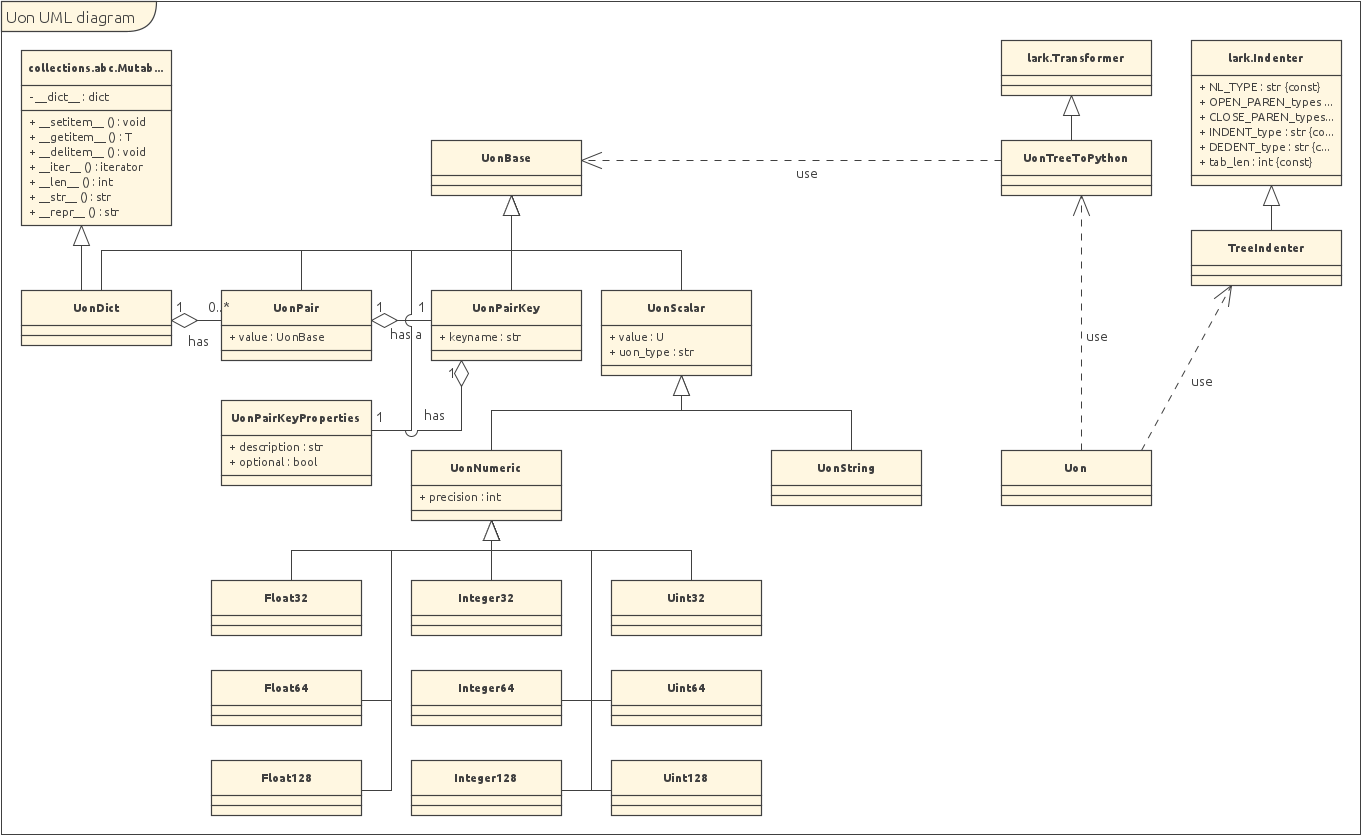
\includegraphics[width=1.0\linewidth]{images/UON/uon_uml.png}
 	\label{fig:uml}
\end{figure}

On the left hand side, we will find all the classes we've defined to represent the different data types of UON values. We will use them to build Python objects from the parse tree when visiting its nodes during transformation. They all inherit from base class \emph{UonBase} which represents the UON type (since everything in UON is a type).

On the right hand side, we see the classes responsible for parsing and transforming namely the \emph{UONTreeToPython} and \emph{TreeIndenter} that you'll find in \\ \emph{uon\_2\_tree\_transformer.py}. They inherit from the lark corresponding classes. And finally we have the \emph{UON} class, which acts as the interface to interact with out parser. It exposes a standard API for data serialization/deserialization (dump and load).

\subsubsection{Indentation}
What distinguishes YAML from other serialization formats or Python from other Programming languages? It's that indentation matters! It denotes structure just as Python uses for delimiting blocks and defining scopes. For example:
\begin{lstlisting}
- 
  - Ophelia
- Hamlet
\end{lstlisting}
is equivalent to a nested list inside a list in Python [['Ophelia'], 'Hamlet']
but 
\begin{lstlisting}
- 
- Ophelia
- Hamlet
\end{lstlisting}
is equivalent to just a list of 3 elements in Python [None, 'Ophelia', 'Hamlet']

So indentation is just a bunch of whitespaces (not tabular characters, YAML states that tabs are a source of ambiguities since different systems treat tabs differently). What does that change for our grammar? Unfortunately, it changes everything.

Indentation is context-sensitive. If you're not convinced, ask yourself how does the parser know that "Ophelia" is a nested list in the first example, and just another list element like in the second example. It's because \textbf{it knows it's surrounded} by an indentation and then a dedentation. That means the result of the parsing is dependent on the context, which here is the indentation.

Denoting blocks using indentation is also called the \textbf{off-side rule}, in contrast to curly-bracket languages where indentation i not meaningful and indent style is only a matter of convention and code formatting (\url{https://en.wikipedia.org/wiki/Off-side_rule}).

How are these off-side rules implemented? (\url{https://docs.python.org/3/reference/lexical_analysis.html#indentation}) In Python this is done during the lexical analysis phase and it usually involves a powerful lexer. When the lexer encounters an increase in indentation, it emits an INDENT token, and when it detects a decrease in indentation, it outputs a DEDENT token. They are the equivalent of opening "\{" and closing braces "\}" when denoting blocks in other languages. However this requires that the lexer hold a state and keep track of the current indentation level. So when it encounters an indentation in the next line, and depending on the current indentation level, it chooses to emit an INDENT or a DEDENT token accordingly. 

\textbf{Handling indentation in Lark}

Fortunately, Lark has a way of handling context-sensitive indentation as well. This involves a postlex stage, where INDENT/DEDENT tokens are manufactured. This means that there two passes, where the first pass is the normal pass of the lexer outputting the tokens according to our grammar, and the second pass concerns the INDENT and DEDENT tokens relevant for indentation. (\url{https://github.com/lark-parser/lark/blob/master/examples/indented_tree.py})

What does that change for our grammar? It means that whitespace and newline suddenly became important and we can't ignore them anymore. And this is going to change the structure of all our grammar.

First we must define what a newline must look like in UON. We define it as such:
\begin{lstlisting}
_NL: /(\r?\n[\t ]*)+/
\end{lstlisting}

Then we declare the INDENT and DEDENT tokens. In lark you can use \emph{\%declare} to declare a terminal in your grammar without defining it. It is useful for plugins or in cases like this one.  

Then you start changing your grammar accordingly. For example for nested collections, we define it as such:

\begin{lstlisting}
_collection: _NL [_INDENT _value _DEDENT]
\end{lstlisting}

A nested collection is defined by an increase in indentation, the value of the collection and then a decrease in indentation.

\textbf{Gentle Reminder}: Rules that start with an underscore are inlined in the parse tree.

After adapting our grammar to handle indentation, we must now let our parser how indentation is done in our language. For that we define our own custom class \emph{TreeIndenter} (found in \emph{uon\_2\_tree\_transformer.py}) that inherits from \emph{lark.Indenter} and we must define the following attributes:
\begin{itemize}
    \item \textbf{NL\_type}: the terminal in our grammar that defines how newlines are represented in our language, namely the \emph{\_NL} we've defined above.
    \item \textbf{OPEN\_PAREN\_types} and \textbf{CLOSE\_PAREN\_types}: The indenter takes also the type of enclosing grammatical structures in our language such as parentheses "()", square brackets "[]" or braces "\{\}". In UON, we expect to use every single one of the aforementioned parentheses types, for example we use normal parentheses for describing UON properties, curly braces for defining mappings, and square brackets for defining ranges. So we add them all to the list of \textbf{OPEN\_PAREN\_types} and \textbf{CLOSE\_PAREN\_types} accordingly:
    
    \begin{lstlisting}[language=python]
    OPEN_PAREN_types = ['LPAR', 'LSQB', 'LBRACE']
    CLOSE_PAREN_types = ['RPAR', 'RSQB', 'RBRACE']
    \end{lstlisting}
    
    And what this does is that the parser can safely handle you writing expressions inside enclosing parentheses spanning multiple lines. How this works is that indenter ignores the newline tokens at the end of these lines and the parsing can proceed normally for the expression inside. Here are the first 3 lines of the method \emph{handle\_NL} of \emph{lark.Indenter.py}. 
    
    \begin{lstlisting}[language = python]
    def handle_NL(self, token):
        if self.paren_level > 0:
            return

        yield token
    \end{lstlisting}
    
    It takes a token from the lexer (since this is a postlex stage), checks if the current parenthesis level is bigger than 0 which is the equivalent of saying that a parentheses type symbol has been opened and has not been closed yet (same logic for indentation/dedent), and if so it returns from the function, which means there is no newline token emitted that can interfere with the parsing of the expression inside the parentheses and would cause it to fail since it’s an unexpected token. Otherwise, it would just emit the newline token.

    \item \textbf{INDENT\_type} and \textbf{DEDENT\_type}: the terminals in our grammar that represent an indentation or a dedent. In our case, these are the new INDENT/DECLARED tokens that we've decalred in our grammar (without defining them).
    \item \textbf{tab\_len}: The length of a tabular character. In our case we define it just for the sake of completeness, but we don't really use, since the use of tabs is discourages.
\end{itemize}

Now we just have to pass this Indenter class to the Lark constructor that generates our parser, to let the parser know that a postlex stage is needed for our language, to handle indentation.

Let's see the result of all this in an example, taken from the YAML spec, where they define a list of two elements, where each element is a mapping of its own:
\begin{lstlisting}[language=Python]
test_indentation = """
-
  name: Mark McGwire
  hr:   65
  avg:  0.278
-
  name: Sammy Sosa
  hr:   63
  avg:  0.288
"""
uon_2_parser = Lark.open(uon_2_grammar_file, parser='lalr',
                         postlex=TreeIndenter(), start='start', debug=True)
uon_parser_2.parse(test_indentation)
\end{lstlisting}

The result parse tree:

\begin{lstlisting}
top_seq
  seq_item
    top_map
      pair
        pair_key
          string        name
        scalar
          string
            Mark
            McGwire
      pair
        pair_key
          string        hr
        scalar
          number        65
      pair
        pair_key
          string        avg
        scalar
          number        0.278
  seq_item
    top_map
      pair
        pair_key
          string        name
        scalar
          string
            Sammy
            Sosa
      pair
        pair_key
          string        hr
        scalar
          number        63
      pair
        pair_key
          string        avg
        scalar
          number        0.288
\end{lstlisting}

\emph{top\_seq} represent a sequence or a list, and \emph{top\_map} represents a mapping. We can see that our parser recognizes properly the nested maps in our list, by the help of indentation.

\subsection{Type coercion}
UON supports a rich set of datatypes. The following represents the structural types.

\begin{figure}[ht!]
 	\centering
 	\caption{UON structural types}
 	\includegraphics[width=1.0\linewidth]{images/UON/structural_types.png}
 	\label{lab:perceptron}
\end{figure}

For now we make do with mappings ans sequences in our parser for UON. But it's eligible to expand it to support more types in the future.

There is also support for numeric datatypes such as float, integer and unsigned integer with different precisions. For a quick overview of the available numeric datatypes, please refer to the UON specification: \url{https://github.com/uon-language/specification/blob/master/spec.md#scalar}.

In our grammar, the type of a uon value is written on the left of the value and is preceded with '!'. For the first version of UON, we're going to parse a selection of these datatypes. We defined terminals for these datatypes, so we can restrain the types that a user can input for a value to the selection of the available types only.
For example:
\begin{lstlisting}
FLOAT_64_TYPE: "!!float64"
INT_128_TYPE: "!!int128"
STR_TYPE: "!!str"
MAPPING_TYPE: "!!mapping"
\end{lstlisting}

For each of these datatypes, we created the corresponding Python classes that represents these datatypes as accurately as possible. Refer to the UML diagram \ref{fig:uml} for these classes. For example, we created a custom \emph{UonDictionary} class, and in order to take advantage of the native dictionary Python data structure, we made \emph{UONDictionary} an implementation of the \textbf{collections.abc} class \emph{MutableMapping}. The \textbf{abc (Abstract Base Classes)} is a module that provides infrastructure for defining abstract classes in Python, and the \emph{collections} module has some concrete classes like \emph{MutableMapping} that represents mappings (another word for it is dictionaries), that we can derive further to add custom behaviour.

We defined as well classes to represent numeric datatypes, and for that we used the excellent \emph{numpy} library to represent different numeric data structures.

We would like to have the ability in UON to coerce between different data types when eligible. For this to happen, the coercion has to \textbf{make sense}. For example, you cannot coerce between a numeric datatype and collection datatype. 

So in the grammar, we separated the collection datatypes from the scalar datatypes, in such a way that only collection-type values can be typed with a structural type (in our case, that's a mapping or a sequence), and scalar-type values can only be typed with scalar-types.

\subsubsection{Coercion in grammar}
An example of a coercion is:
\begin{lstlisting}
d : !!int64 !!float32 63.7
\end{lstlisting}
63.7 which is recognized as a \emph{Float64} by the grammar, is coerced into \emph{Float32} and then to \emph{Integer64}. The coercion is applied from right to left (thus type coercion is a  right-associative operation)This type of coercion is what we call 
\textbf{implicit coercion}.
That means that we set the types and the coercion is done implicitly.

For now, type coercion is only considere between numeric datatypes. To express the right-associativity of type coercion in the grammar, we define a rule \emph{typed\_scalar}:
\begin{lstlisting}
typed_scalar : scalar_type  (typed_scalar | _scalar_value)
\end{lstlisting}
which is a scalar type succeeded by either:
\begin{itemize}
    \item \emph{\_scalar\_value} in which case the coercion is applied directly on the scalar value
    \item or another \emph{typed\_scalar} in which case the coercion is applied recursively to the right 
\end{itemize}
You can verify by writing the rule this way, the coercion operation is right-associative.

As for the actual coercion, this is done in the \emph{UON2TreeToPython} tranformer. The \emph{typed\_scalar(self, value)} method returns a scalar coerced. The result is returned to the next typed scalar up the stack and so on. 

For type coercion between numeric datatypes, we use \emph{numpy} constructors. That constructor is used when creating our own defined UON numeric Python objects (subclasses of \emph{UonNumeric in the UML \ref{fig:uml}}) in the first place. Finally, we defined a dictionary in \emph{type\_coercion.py}, where every numeric datatype is mapped to the corresponding constructor of our Python UON numeric classes.

\subsubsection{Coercion example}
Given the following input:
\begin{lstlisting}[language=Python]
test_type_coercion = """
a : !!int32 !!float64 58767638927.4
"""
\end{lstlisting}

We get the following parse tree
\begin{lstlisting}
top_map
  pair
    pair_key
      string    a
    scalar
      typed_scalar
        scalar_type     !!int32
        typed_scalar
          scalar_type   !!float64
          number        58767638927.4
\end{lstlisting}

and the result of the transformation:
\begin{lstlisting}
{a : !!int32 -2147483648}
\end{lstlisting}
We can see the parse tree keeping all the information on the types involved in the upcoming type coercion. After the transformation, the coercion from float64 to integer32 is applied and we get a 32 bit integer -2147483648 which is a clear case of integer overflow when converting 58767638927.4 to a 32 bit integer.

[TO BE CONTINUED]

\subsection{UON 2 parser challenges}
Here are some of the challenges and tricky stuff encountered when implementing a parser for UON 2.

\subsubsection{Parsing Strings}
One problem I had was parsing between scalar values, namely strings and numbers.
I defined a STRING terminal and defined it as a match to a regex :
\begin{lstlisting}
STRING :  /[^-:#()\[\]{}\n\d]+/
\end{lstlisting}
Which is any character except the special characters included in the negated set [\^...]. This includes whitespace of course to match a string and not just words. I kind of naively put `\\n` newlines in my negated set so the strings do not match newlines, given how important they are as separators in my grammar. This means that all strings in a uon file must be written on the same line, which is unacceptable. Hence the need for block style strings like YAML (literal starting with ‘|’ or folded style ‘>’).
Another naive pattern I’ve put in the negated set was ‘\\d’ for digits. I didn’t want my strings to match numbers, to separate between numbers and strings. This means that a string cannot contain numbers, which is also not desirable behaviour and that’s what we are going to try to solve here.

\textbf{1st Attempt: Introduce strings as list of words}

One solution was to include whitespace `\\s` in the negated set of STRING and rename the terminal to WORD, then introduce a rule string as a list of words as such:
\begin{lstlisting}
WORD:  /[^:#()\[\]{}\n\"\'\s]+/
string : WORD+
\end{lstlisting}
Note that we also removed the digit character set from the negated set in \emph{STRING}, now called \emph{WORD} so that \emph{WORD} can match numbers. Now a string can contain numbers as well. Take a look at this example:

\begin{lstlisting}[language=Python]
test_uon_strings = """
a : I put numbers 28.5 in my string but this should still be parsed as a string
b : 28.5
"""
\end{lstlisting}

With the current version of the grammar this will be parsed as such:
\begin{figure}[h!]
 	\centering
 	\caption{1st attempt at parsing strings}
 	\includegraphics[width=0.3\linewidth, height=8cm]{images/Problems/string_words.png}
 	\label{lab:perceptron}
\end{figure}

Note how the parser correctly parsed the string of the value of key `a` as a list of words including the “28.5”, but parsed the 28.5 in key `b` as a number. How did the parser solve this ambiguity? Recall that a scalar is defined as such :
\begin{lstlisting}
scalar : (string | number) _NL+
\end{lstlisting}
So it’s either a \emph{string} which is a list of \emph{WORD}s or a \emph{number} followed by at least one newline. So if he parses a \emph{number} instead of a \emph{WORD} in the middle of a string, he will have a list of words and numbers which fits neither \emph{string} nor \emph{number} in \emph{scalar}. The only choice he has is to parse the number in a list of words as a word as well which fits the rule of \emph{string}. 

But what if the number comes at the beginning of a string like so:
\begin{lstlisting}(language=Python)
test_uon_strings = """
a : 28.5 I put numbers 28.5 in my string but this should still be parsed as a string
b : 28.5
"""
\end{lstlisting}
He will immediately see a number “28.5” and parse it as a \emph{number}, since our parser is a LALR parser. How do we solve this ambiguity?

\textbf{2nd  Attempt : Redefine string rule
}
We can redefine the string rule, to take care of the case where a string could start with a number as such:
\begin{lstlisting}
string :  number WORD+ | WORD+
 
number : DECIMAL | FLOAT_NUMBER
DECIMAL : /0|[1-9]\d*/i
FLOAT_NUMBER: /((\d+\.\d*|\.\d+)(e[-+]?\d+)?|\d+(e[-+]?\d+))/i
\end{lstlisting}
Keeping the \emph{WORD} terminal from before, a string can start with a number in which case it must be followed by at least one word so it could qualify as a string, or it can be a simple list of words as before. We would expect this to work, but with every modification we do in our grammar rules, it will almost always have a repercussion somewhere else. When we try to parse with the following input 

\begin{lstlisting}[language=python]
test_strings = """
a : 28 should be parsed as string
b : 28
"""
\end{lstlisting}

with our current definition of \emph{string} we get:

\begin{figure}[h!]
 	\centering
 	\caption{2nd attempt at parsing strings}
 	\includegraphics[width=0.3\linewidth]{images/Problems/test_strings_2nd_attempt.png}
 	\label{lab:perceptron}
\end{figure}
We can see all numbers parsed as strings now. What’s interesting is that the first production rule of \emph{string}, namely \emph{number WORD+}, is never produced otherwise we would see in the output a number node "number 28" inside the string. It’s always the second rule, namely \emph{WORD}+ which is a list of words that is produced and that means that the numbers literals like 28 are matched as \emph{WORD} and not \emph{DECIMAL} or \emph{FLOAT\_NUMBER}. We can probably guess why, it’s because the \emph{WORD} can also match number literals, as we intended it to be able to have numbers inside strings. That means the number terminals and \emph{WORD} are colliding. So why does the lexer match 28 as \emph{WORD} instead of \emph{DECIMAL} or \emph{FLOATING\_POINT}?

\textbf{Solution: Grammar lexer priorities
}
Remember that you can assign priorities to Lark grammar terminals? That means that when lexing our input, the lexer will match the literal with the highest priority first. If not specified for a terminal, a terminal has a priority 1 by default. So our \emph{WORD} and our terminals that constitute the production rules for our \emph{number}, namely \emph{DECIMAL} AND \emph{FLOAT\_NUMBER}, all have the same priority. What happens if the lexer meets an input literal like “28.5” and priorities of \emph{WORD} and the number terminals match? It will match the literal according to the following precedence:
\begin{enumerate}
    \item Highest priority first (priority is specified as: TERM.number: ...)
    \item Length of match (for regexps, the longest theoretical match is used)
    \item Length of literal / pattern definition
    \item Name
\end{enumerate}
The length of match and the length of the literal are the same for an input literal like “28.5” so it all comes down to the name of the terminal! \emph{DECIMAL} and \emph{FLOAT\_NUMBER} come before \emph{WORD} name-wise. That’s why the match with \emph{WORD} comes first. But if our \emph{WORD} terminal was named \emph{BLA} for example, then the lexer will try to match \emph{DECIMAL} or \emph{FLOAT\_NUMBER} first, and our problem would be solved.

But this sounds like a really hacky way to solve this problem, and \emph{BLA} doesn’t evoke much about what the terminal represents, which is a word. A better way would be to give a higher priority to number terminals as so:
\begin{lstlisting}
number : DECIMAL | FLOAT_NUMBER
DECIMAL.2 : /0|[1-9]\d*/i
FLOAT_NUMBER.2: /((\d+\.\d*|\.\d+)(e[-+]?\d+)?|\d+(e[-+]?\d+))/i
\end{lstlisting}

Now number terminals have a higher priority of 2 instead of one like\emph{WORD}, and when a lexer sees a number literal like “28”, it will match a \emph{DECIMAL} not a \emph{WORD}.

\textbf{Note from the author of Lark:} After asking the author of Lark on this approach, he said that it would be better to keep the grammar as before and instead “disambiguate post-parse. Increasing the priority on the number will cause strings to be misidentified as numbers, because the parser can't see what comes after”. And he’s right. Increasing the priorities on number terminals made a string that starts with a number like the example above be parsed as such \ref{fig:author note}.

\begin{figure}[ht!]
 	\centering
 	\caption{Author note}
 	\includegraphics[width=0.3\linewidth]{images/Problems/note_author_test_string.png}
 	\label{fig:author note}
\end{figure}

The string node will have a \emph{number} 28 node at the beginning since priorities now lie with number terminals and not \emph{WORD}. And it’s up to me during post-parse to convert this number node to a string, given it’s inside a string node.
His initial suggestion would be to let go of the \emph{number} rule, and have numbers parsed as strings. Then during post-parse, which is when I visit the nodes of my parse tree, I should parse the strings as numbers. If the parsing works, then the string was effectively a number. If not then it was a normal string. 
I prefer my approach, since I’d rather convert a number to string, than parse a string to a number, and then check if it’s valid. But he’s right in the sense that one way or another, I would have to resolve this ambiguity post-parse.


\subsubsection{UON dictionary}
You might’ve noticed that there was something the way we constructed the uon dictionaries after parsing and visiting the tree nodes. The \emph{dict()} method receives a list of tuples, which are the key-value pairs of that dictionary node in the parse tree, and constructs a \emph{UonDictionary} with it. There is nothing unusual here. The oddity however is how we construct the key-value tuple. When we encounter a pair node in our parse tree, which represents a key-value pair, we return the following:

\begin{lstlisting}[language=Python]
def pair(self, pair):
       print("visiting pair: ", pair)
       return pair[0].keyname, UonPair(pair[0], pair[1])
\end{lstlisting}

We construct a \emph{UonPair} using the key and the value from the pair argument and then we return a tuple constructed of the pair key keyname and the \emph{UonPair} itself! Why? Because this would make searching our dictionaries easier using only the keyname of the pair, which is a string. Remember that a \emph{Pair} consists of a \emph{PairKey} which encapsulates the pair keyname and its properties, and on the other hand the value of that pair. And that \emph{PairKey} is an object, which has to be hashable, and isn’t very convenient in searching our UonDictionary. Keys that are strings are more convenient for searching. And that is why we created the \emph{Pair} class in the first place, it encapsulates the \emph{PairKey} - containing the properties of that pair -  and the value of that pair. 

Otherwise we could have just provided that tuple simply using those two elements instead as such:
\begin{lstlisting}[language=Python]
def pair(self, pair):
       print("visiting pair: ", pair)
       return (pair[0], pair[1])
\end{lstlisting}

Note that pair[0] contains the \emph{PairKey} instance, and pair[1] contains the value. But that means that the key of a key-value pair in our dictionary will be a \emph{PairKey} object and that is not very convenient for searching. After all, we know our \emph{UonDictionary} object is a custom dictionary class that derives from the abc class \emph{MutableMapping} but the core functionalities like the search and setting and deletion functions remain virtually the same. If we’d like \emph{PairKey}s objects to serve as our keys, we would have to construct that object first and then use it for searching, which means we would have to provide a hash function on \emph{PairKey} objects and we would have to define how \emph{PairKey} objects can be equal. 

TODO: provide example

The more convenient option would be to provide the possibility to search by only the keyname. That means we have to override the built-in \emph{\_\_getitem()\_\_} method of UonDictionary and provide a custom implementation ourselves that does a linear search on our set of keys using only the keyname and check if that keyname and the keyname of a PairKey correspond, and then return the value if they do. But then we would be losing the full efficiency of the build-in \emph{getitem()} search method of the python dictionaries.

\pagebreak

\section{Planning \& Current Roadmap}

\subsection{Gantt shart}
Here is the Gantt shart for this project. This shart has been heavily updated during the semester, to take into account the changes in the tasks and the fact that certain tasks were unknown beforehand, as well reorganizing my hours. 

As mentioned before, this project was designed to be implemented in increments. Previous tasks consistenly have to be revisited to adapt to the new features introduced for UON. The task that took the most time by far was writing the grammars. 

\includepdf[pages=-]{images/Planning/UON_Gantt_shart.pdf}

\subsection{Current Roadmap}
Now that we've reached the intermediary report checkpoint, it's good to do a quick overview of the current situation and evaluate what can be done with the time left.

With the current status of the project, we have a functional UON 2 grammar that is extendible. We have a parse tree and a transformer that successfully transforms the result of the parse into Python Objects. We have defined UON types, also easily extensible, and we managed to construct them, with respect to the parse tree nodes. 

We now have to focus on the validation schema, one of UON's important features. Validation schemas rely heavily on UON properties. We might have to rework how properties are implemented and how they are stored in the resulting Python UON object, to be able to run validation through. Right now, properties like description or optional are part of the \emph{UONPairKeyProperties}. 

Up until now we've been focusing mainly on parsing UON, that is deserializing a UON input. Next step is to serialize Python objects. We have to think about the structure of a Python object. Just as we established a correspondence between UON data structures and Python native data structures, we now have to do it the other way around.

Another important aspect that is missing, one that I'm not proud of as a developer, is unit testing. The constant changing nature of the grammar forced me to drop unit testing for now since any major (or sometimes minor) changes in the grammar yield different results in the parsing and would lead to rewriting a lot of those unit tests. All I do for now is keep sample UON inputs, and do manual tests to verify the output.

There is a lot to do. But a lot of the initial building blocks are here, and a certain work methodology has been established.

\pagebreak

\subsection{Binary Serialization}
[TODO]

\pagebreak

\subsection{Schema Validation}
[TODO]

\pagebreak

\section{Conclusion}
[TODO]

\pagebreak

\section{What next?}

\pagebreak

\section{Bibliography \& Resources}
[1] \url{https://medium.com/@dilankam/java-serialization-4ff2d5cf5fa8 serialization image}
 
[2] \url{https://stackoverflow.com/questions/36767310/why-is-json-faster-than-bson-in-node-js} 

[3] \url{https://www.json.org/json-en.html} 

[4] \url{https://yaml.org/} 

[5] \url{https://github.com/yaml/yaml-grammar} 

[6] \url{https://www.w3.org/2003/08/binary-interchange-workshop/29-MicrosoftPosition.htm} 

[7] \url{http://bsonspec.org/spec.html} 

[8] \url{https://www.mongodb.com/json-and-bson} 

[9] \url{https://developers.google.com/protocol-buffers} 

[10] \url{https://developers.google.com/protocol-buffers/docs/proto#scalar} 

[11] \url{https://en.wikipedia.org/wiki/Comparison_of_data-serialization_formats}

[12] \url{https://github.com/lark-parser/lark}

[13] \url{https://lark-parser.readthedocs.io/en/latest/philosophy/}


\end{document}